\def\ratioGraphiqueX{0.75} 
\def\ratioGraphiqueY{0.6}
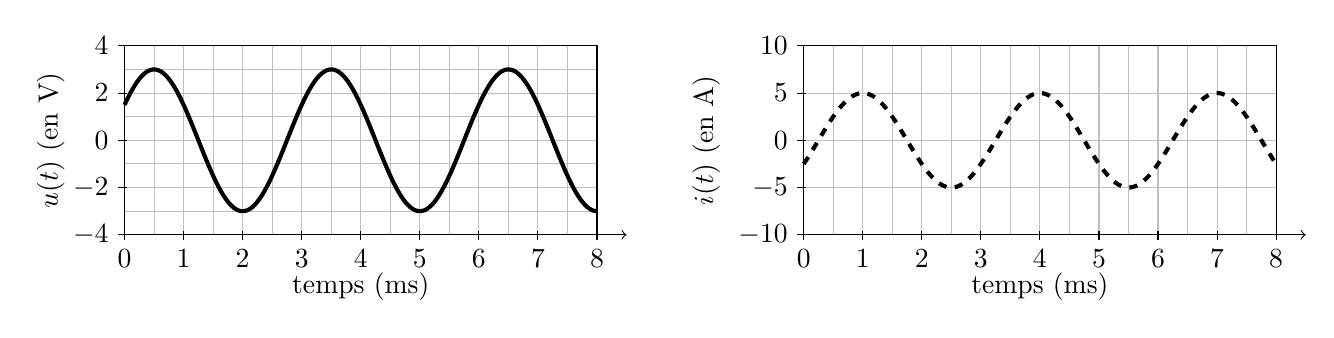
\begin{tikzpicture}[xscale=\ratioGraphiqueX, yscale=\ratioGraphiqueY]
\shorthandoff{:!}
\begin{scope}
	\draw[xstep=0.5cm,ystep=0.5cm,color=gray!50](-4,-2) grid (4,2);
	\draw(-4,-2) rectangle (4,2);
	\draw[->] (-4,-2) -- (4.5, -2);% node[below right] () {temps (en \si{ms})};
	\foreach \x in {0,...,8}
     		\draw (\x-4,-2cm+2pt) -- (\x-4,-2cm-3pt)
			node[anchor=north] {\x};
	\foreach \y in {-4,-2,...,4}
     		\draw (-4cm+1pt,\y/2) -- (-4cm-3pt,\y/2)
			node[anchor=east] {$\y$};
	\draw(0,-3.1)node[]{temps (\si{ms})};
	\draw(-5.25,0)node[rotate=90]{$u(t)$ (en \si{V})};
	%\draw [domain=-4:4,samples=500,line width=1.5pt] plot (\x,{1.5*cos(2*pi/3*(\x+1) r)});
	%\draw [domain=-4:4,samples=500,line width=1.5pt] plot (\x,{1.5*cos(2*pi/3*(\x+2) r)});
	%\draw [domain=-4:4,samples=500,line width=1.5pt] plot (\x,{1.5*cos(deg(2*pi*\x/3+pi/4))});
	\draw [domain=-4:4,samples=500,line width=1.5pt] plot (\x,{1.5*cos(deg(2*pi*\x/3+pi/3))});
\end{scope}

\begin{scope}[shift = {(11.5,0)}]
	\draw[xstep=0.5cm,ystep=8cm,color=gray!50](-4,-2) grid (4,2);
	\draw[color=gray!50] (-4,-1) -- + (8,0);
	\draw[color=gray!50] (-4,1) -- + (8,0);
	\draw(-4,-2) rectangle (4,2);
	\draw[->] (-4,-2) -- (4.5, -2);% node[below right] () {temps (en \si{ms})};
	\foreach \x in {0,...,8}
     		\draw (\x-4,-2cm+2pt) -- (\x-4,-2cm-3pt)
			node[anchor=north] {\x};
	\foreach \y in {-10,-5,...,10}
     		\draw (-4cm+1pt,\y/5) -- (-4cm-3pt,\y/5)
			node[anchor=east] {$\y$};
	\draw(0,-3.1)node[]{temps (\si{ms})};
	\draw(-5.65,0)node[rotate=90]{$i(t)$ (en \si{A})};
	%\draw [dashed,domain=-4:4,samples=500,line width=1.5pt] plot (\x,{1.5*cos(deg(2*pi*\x/3+7*pi/12))});
	\draw [dashed,domain=-4:4,samples=500,line width=1.5pt] plot (\x,{1*cos(deg(2*pi*\x/3))});
\end{scope}
\shorthandon{:!}
\end{tikzpicture}